\chapter{Hyperkinetic movement disorder analysis}
\label{ch:nemo}

\textit{
In this chapter we present a real world application for the dynamic projection methods introduced in \cref{ch:proj-eval,ch:proj-algo} in the context of hyperkinetic movement disorder analysis. These disorders manifest in form of abnormal involuntary movements that highly affect the quality of life of the people that suffer from them. These involuntary movements may show regular and rhythmic tendencies, as in tremors; swift ``lightning-like'' jerks or twitches, as in myoclonus; sustained and repetitive movements resulting in abnormal postures, as seen in dystonia; they may present a random, brief, and non-rhythmic character, as in chorea; or can be temporarily suppressible jerks, as in tics.
The diagnosis of these disorders is carried out via careful professional observation and can be extra challenging due to the circunstantial appeareance of certain behaviours (trigged by a specific postures or tasks) and their manifestation via multiple types of movements, which may include a combination of the various hyperkinesias. It is common for medical professional diagnosis to disagree given the complex nature of the disorders.
In this chapter we describe how we transform the data collected during clinical experiments to create a powerful reasoning tool using spectral analysis and temporal dimensionality reduction. 
}

\vspace{5mm} %5mm vertical space

% Myoclonus-Dystonia (M-D) is a movement disorder characterized by a combination of rapid, brief muscle contractions (myoclonus) and/or sustained twisting and repetitive movements that result in abnormal postures (dystonia).

% Myoclonus-dystonia is a movement disorder that typically affects the neck, torso, and arms. Individuals with this condition experience quick, involuntary muscle jerks or twitches (myoclonus). About half of individuals with myoclonus-dystonia develop dystonia, which is involuntary tensing of various muscles that causes unusual positioning. In myoclonus-dystonia, dystonia often affects one or both hands, causing writer's cramp, or the neck, causing the head to turn (torticollis).

% These excess movements can be regular and rhythmic, as in tremor; more sustained and patterned, as in dystonia; brief and random, as in chorea; or jerk-like and temporarily suppressible, as in tics. Diagnosis of the specific condition depends primarily upon careful observation of the clinical features [1]. Tics are the most common hyperkinetic disorder in children. Dystonia, stereotypies, choreoathetosis, tremors, and myoclonus also occur but are less common. Many hyperkinetic movement disorders manifest with multiple types of movements, which may include a combination of the various hyperkinesias.


\eduardo{This in an initial report, not necesarily what the chapter/paper will look like. It is supposed to help me think about how to write about this project and guide me through preliminary patient data analysis.
\\
In the introduction and initial sections we will need to: \\
1 - introduce hyperkinectic movement disorders \\ 
2 - talk about how their manisfestation in different people can differ wildly and how that makes them challenging to classify/diagnose even for medical especialists. \\
3 - talk about our goals creating this visual exploration tool and how this differs from a more traditional supervised learning approach. \\
\\
What are these goals exactly? And what are the pros/cons over what ziuz is doing (list them here...) 
\\
\\
After that we'll probably need a section introducing the different disorders and possibly explaining how they manifest in some of the tasks for illustration. \\
One thing that I'm not sure about is how familiar we expect the reader to be about these disorders.
\\
Then I think we should start to describe our contribution. And I would start by (1) describing the data itself and all the choices/transformations we make along the way until we get to the dynamic projection. 
\\
This includes: \\
\\
1 - Showing what the RAW data looks like \\
1.1 - General description of the experiment, including the tasks, sensor types, and possibly the different disorders (which must be introduced in a previous section). \\
1.2 - Show 3 axis acceleromenter plot for 3 patients (e.g. healthy vs tremor vs chorea) \\
1.3 - Show spectrogram, interpret it, and talk about synchosqueezing \\ 
1.4 - Show how we get that spectrogram into a 'projectable' format: binning of the freqs + sliding window (width, stride) \\
1.5 - Show initial projections --  not sure what data to use here, maybe the 3 patients from before? Probably a more meaningful subset of the data would be better. Right now we have G-PCA, G-tSNE, and PCD-tSNE implemented. Explain dynamic projections and why they are useful and suitable for this application. Maybe do a trail vs single point comparisson.
\\
\\
Next we need to move into data exploration, where we want to find examples of when dynamic projections can bring us insights into the data dynamics and the high dimensional space. Here we will be interested in looking for clusters, outliers, erratic/regular behavior, failures in the data collection, etc.
\\ 
}

\eduardo{CODE: Check code to make sure I can switch sensors (DONE) and that I can 'stack' more than one sensor (NOT DONE))}

\noindent \textbf{Abstract:}

\section{Introduction}

\section{Related work}

\section{Hyperkinectic movement disorders and experiment design}

\section{Our approach (not sure what to call this section)}

\begin{figure*}[ht]
\centering
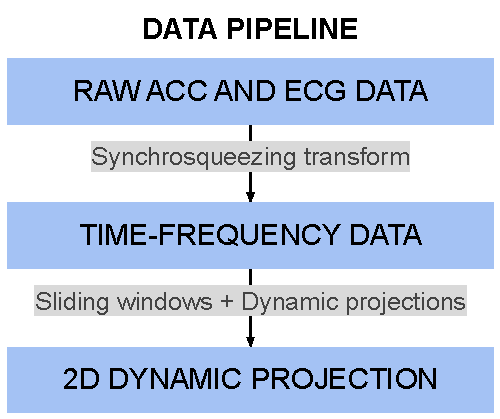
\includegraphics[width=.5\linewidth]{figures/nemo/simple-pipeline.pdf}
\caption{Data transformation.}
\label{fig:nemo-pipe}
\end{figure*}


\begin{figure*}[ht]
\centering
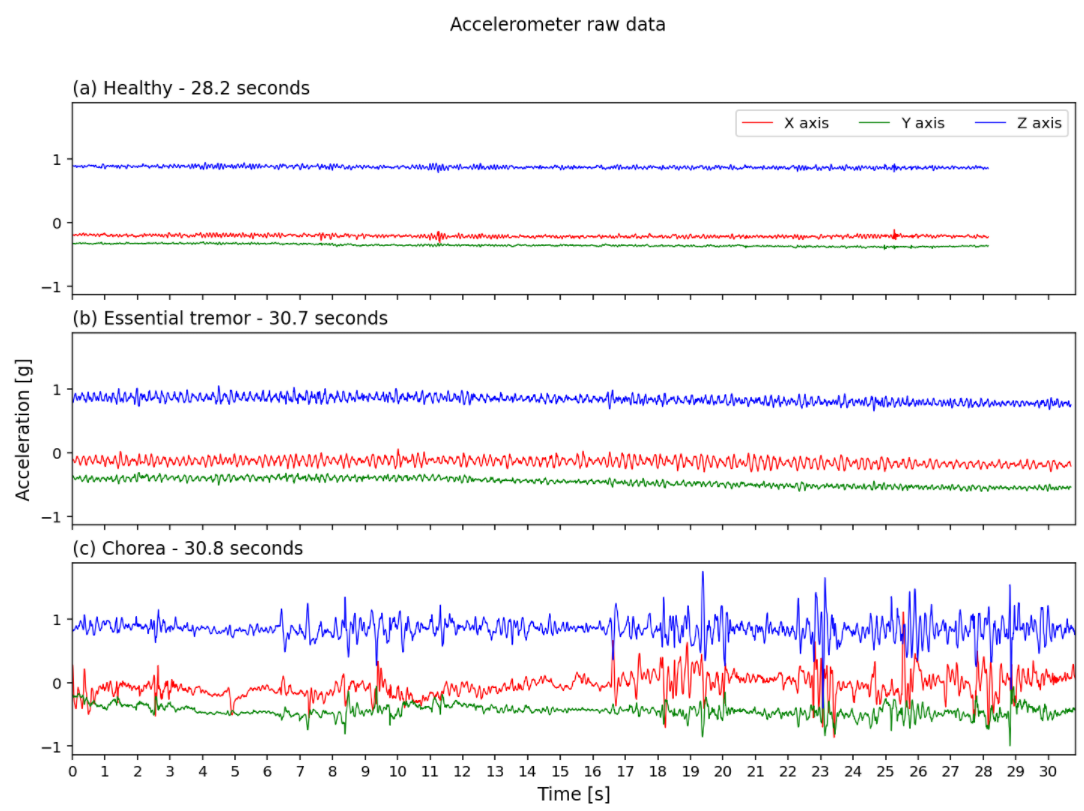
\includegraphics[width=\linewidth]{figures/nemo/acc2.png}
\caption{Accelerometer data for 3 subjects classified by experts as (a) healthy, (b) diagnosed with essential tremor, and (c) diagnosed with chorea. The data corresponds to a task where the subject must hold their hands as still as possible in the position suggested in Fig. \ref{fig:hands}.
Each subplot corresponds to the accelerometer data collected during the experiment and broken down into 3 orthogonal components (X, Y, and Z axis). \eduardo{Are we allowed to upload censored videos to a website?}}
\label{fig:acc}
\end{figure*}


\begin{figure*}[ht]
\centering
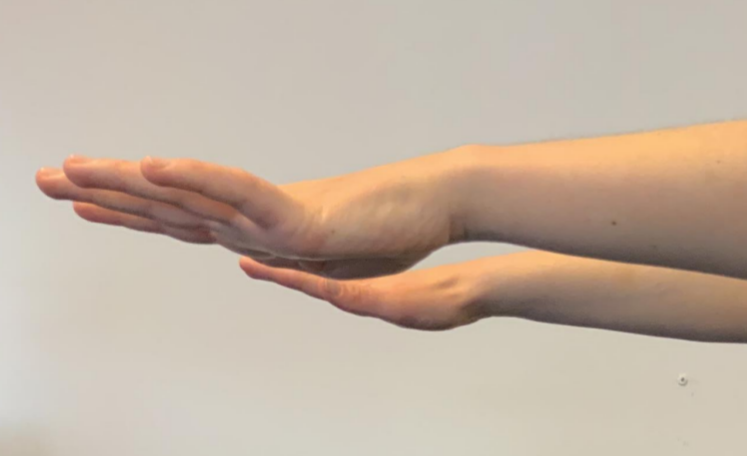
\includegraphics[width=.5\linewidth]{figures/nemo/hands.png}
\caption{Static position with arms and hands streched out in front of body for 20-30 seconds.}
\label{fig:hands}
\end{figure*}


\begin{figure*}[ht]
\centering
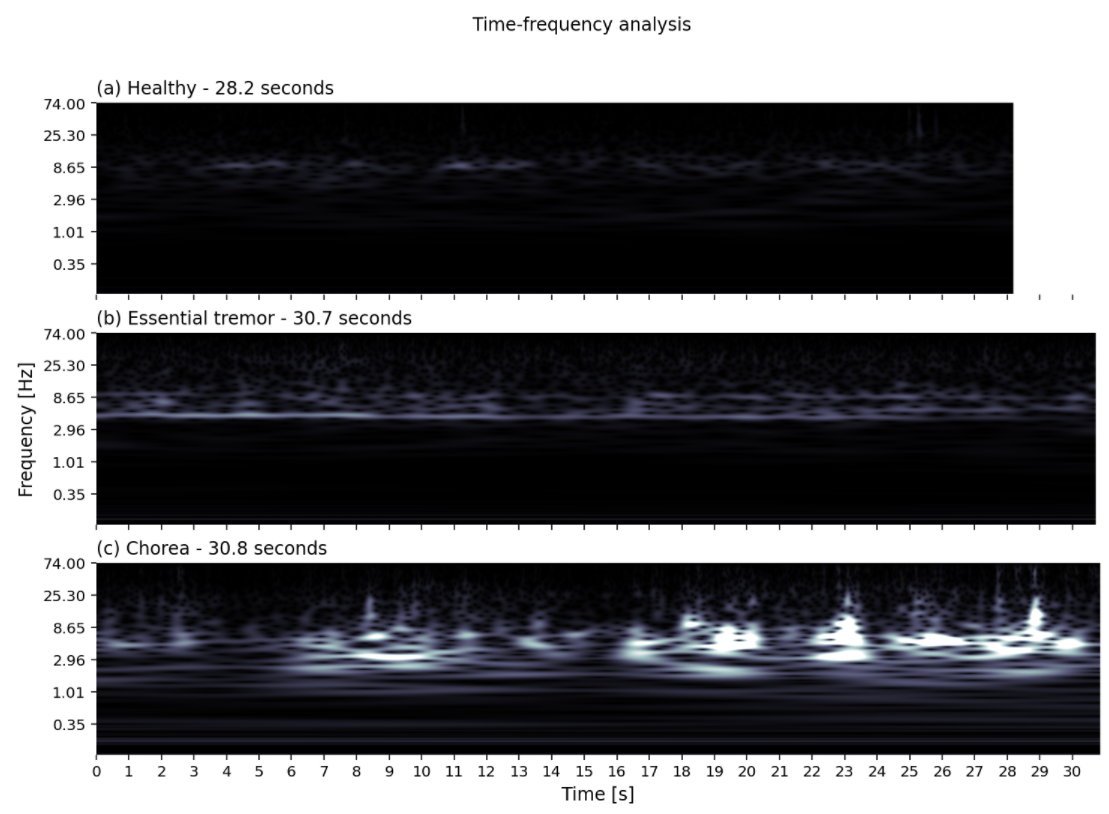
\includegraphics[width=\linewidth]{figures/nemo/freq2.png}
\caption{Time-frequency representation of the acceleration of the Z axis (blue) in Fig. \ref{fig:acc}. Light colors represent high energy in the spectral distribution, i.e., there is a large amplitude component in the subject's movement associated to a particular frequency or frequency distribution.}
\label{fig:freq}
\end{figure*}

\begin{figure*}[ht]
\centering
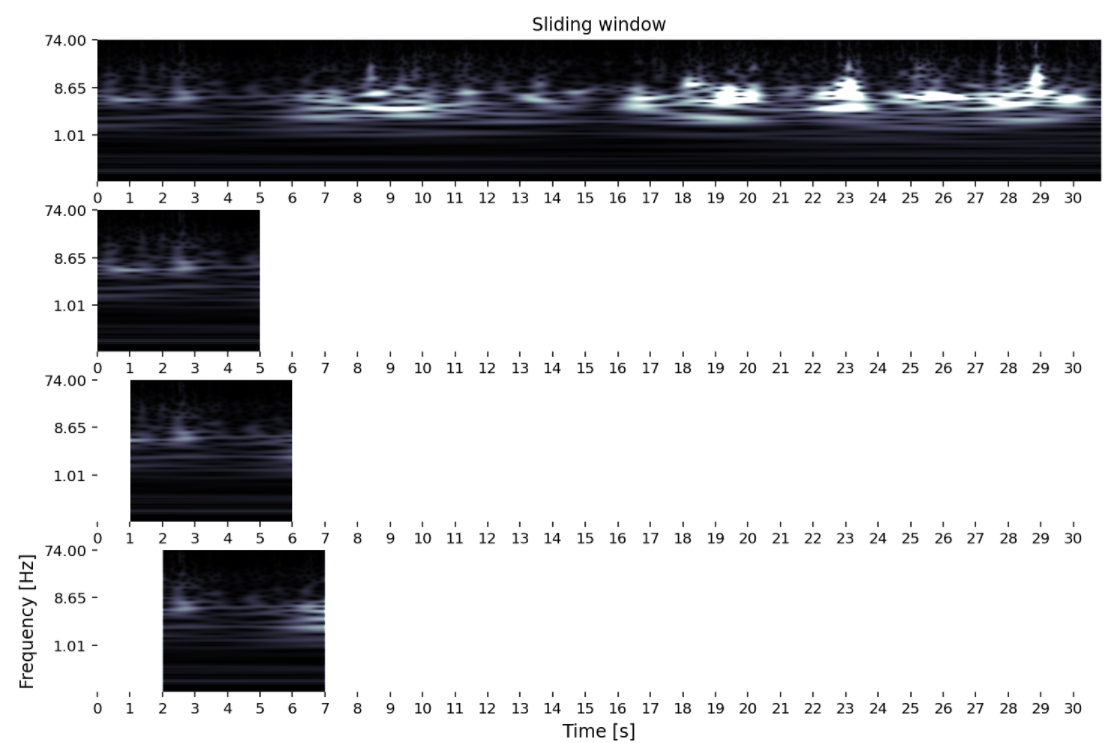
\includegraphics[width=\linewidth]{figures/nemo/sliding.png}
\caption{Before we project our data, we subdivide each spectrogram using the Sliding Window method. In this example, we use a window width of 5 seconds and a stride of 1 second to partition the data from Fig. \ref{fig:freq}c.}
\label{fig:sliding}
\end{figure*}


\begin{figure*}[ht]
\centering
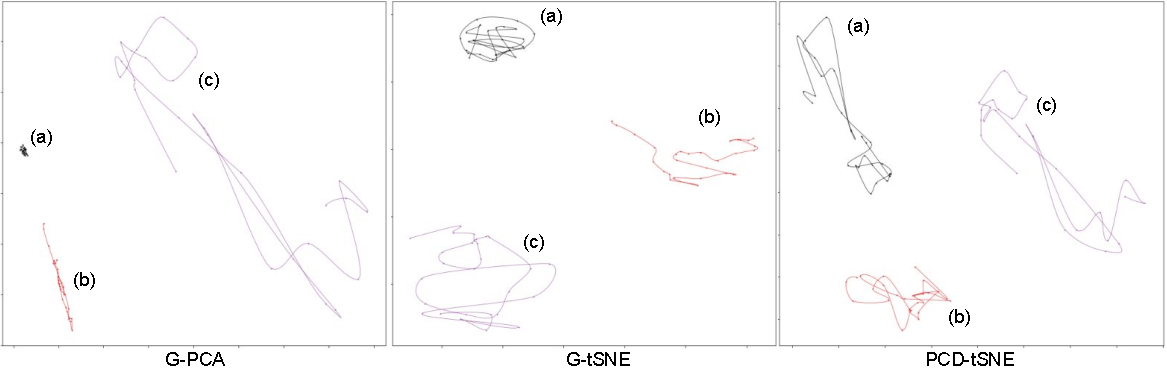
\includegraphics[width=\linewidth]{figures/nemo/nemo1-projections.pdf}
\caption{The last step of the pipeline is to project (using dynamic methods) the data that has been subdivided by the Sliding Window method. Our tool supports 3 dynamic projection methods: G-PCA, G-tSNE, and PCD-tSNE. We visualize the dynamic projections as trails, where we connect the consecutive ``windows''. The data corresponds to the patients presented in \cref{fig:acc,fig:freq}.}
\label{fig:nemo1-projections}
\end{figure*}


\section{Data exploration}

\eduardo{We will limit the analysis to a very small subset of the data (for now). \\
Only one task -- the same as described above --, only one sensor/sensor axis (right hand Z), and only healthy vs tremor patients.} 

\begin{figure}
\centering
\begin{minipage}{.47\textwidth}
    \centering
    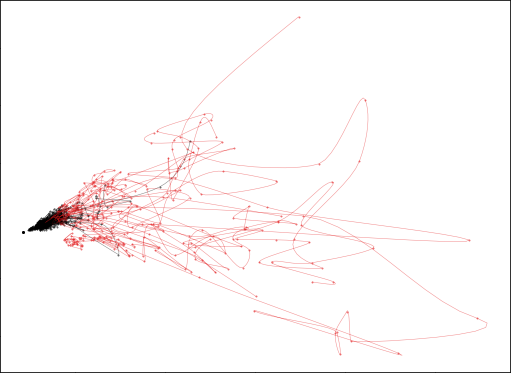
\includegraphics[width=\linewidth]{figures/nemo/exp1.png}
    % \captionof{figure}{A figure}
    \label{fig:exp1-gpca-1s-1s}
\end{minipage}%
\begin{minipage}{.47\textwidth}
    \centering
    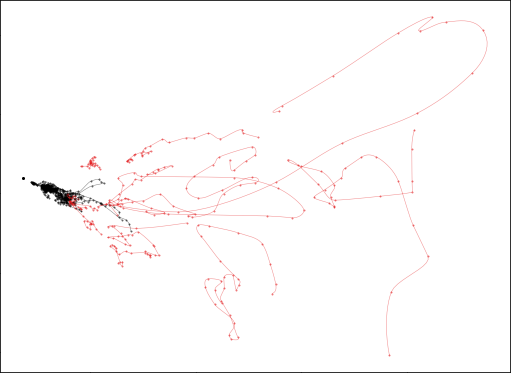
\includegraphics[width=\linewidth]{figures/nemo/exp1-5s-window.png}
    % \captionof{figure}{Another figure}
    \label{fig:exp1-gpca-5s-1s}
\end{minipage}
\caption{G-PCA projection of 24 healthy (black) and 11 tremor (red) patients with window width and stride of [1s, 1s] on the left and [5s, 1s] on the right.}
\end{figure}

\begin{figure*}[ht]
\centering
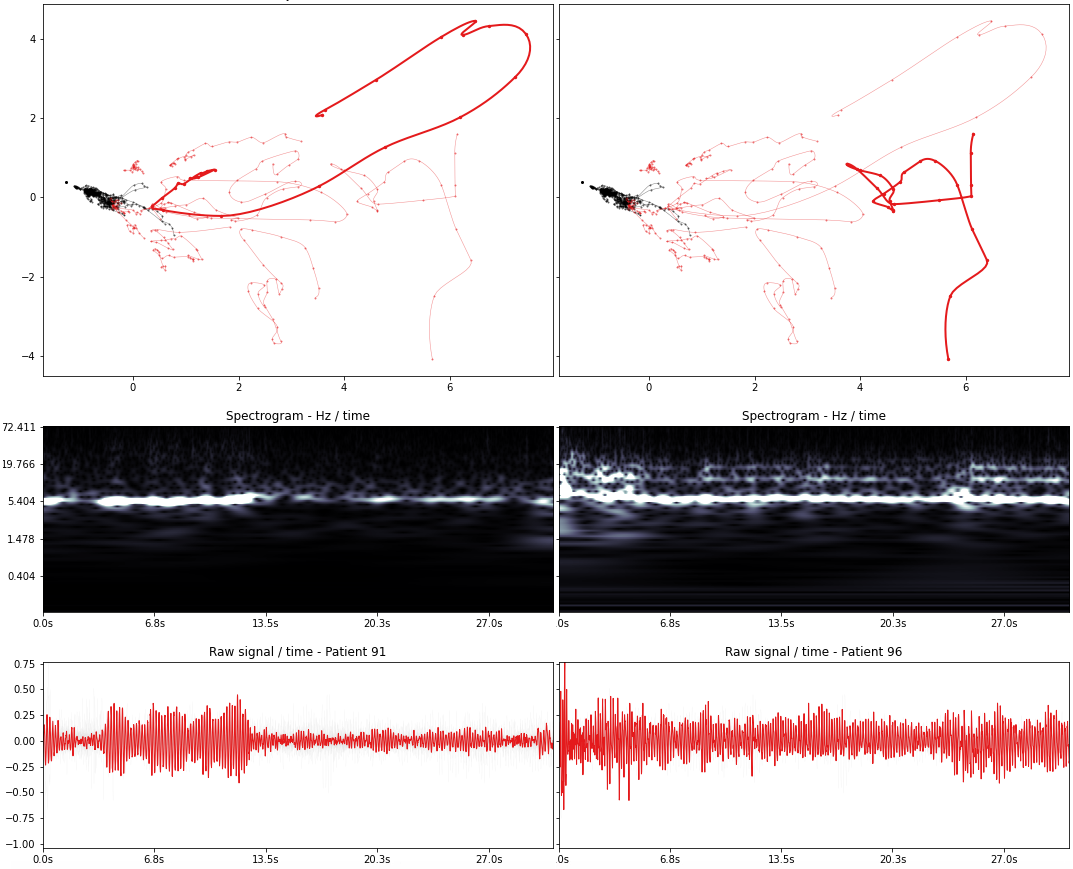
\includegraphics[width=\linewidth]{figures/nemo/exp1-9196.png}
\caption{}
\label{fig:exp1-9196}
\end{figure*}

\begin{figure*}[ht]
\centering
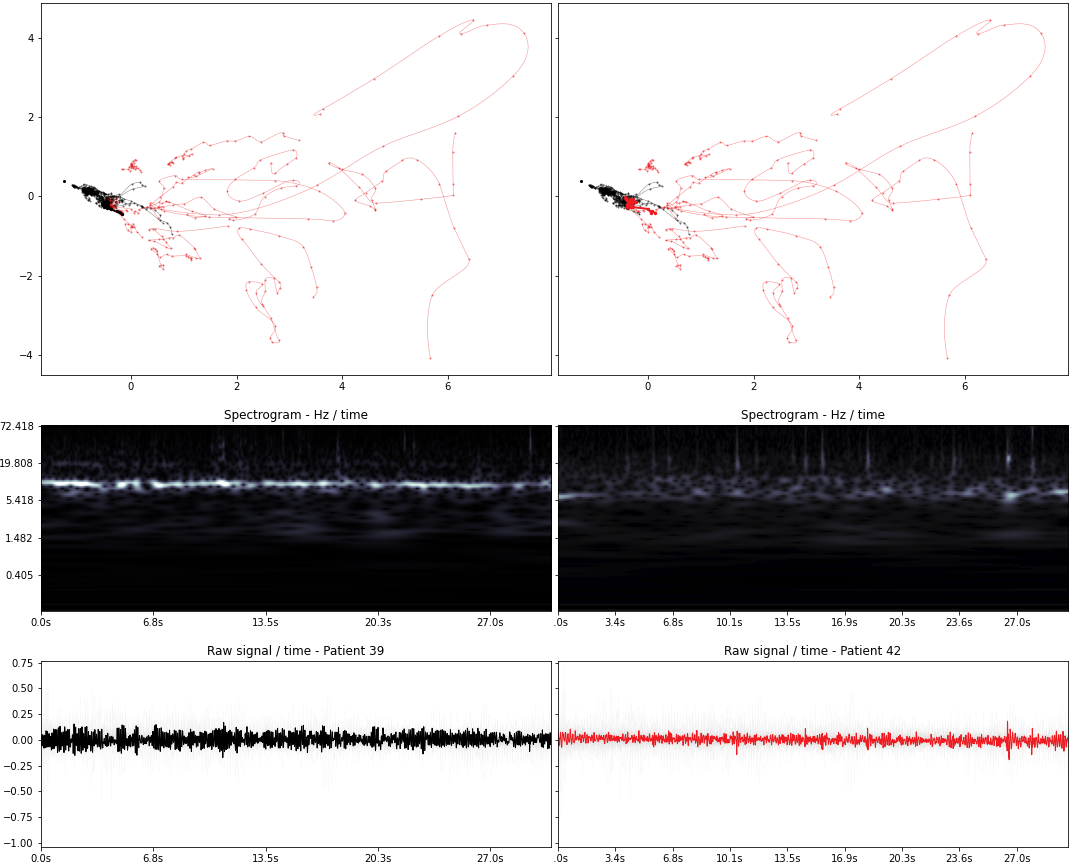
\includegraphics[width=\linewidth]{figures/nemo/exp1-3942.png}
\caption{The trail representing the patient on the right is very close to the healthy group. If we look at only his right hand during the recording of this specific task, it is hard to tell that he/she suffers from tremors and it raises the question as to why was he/she diagnosed with tremors. Does it have a postural aspect to it that isn't captured in this task or perhaps it only appears in certain circunstances?}
\label{fig:exp1-3942}
\end{figure*}

\begin{figure*}[ht]
\centering
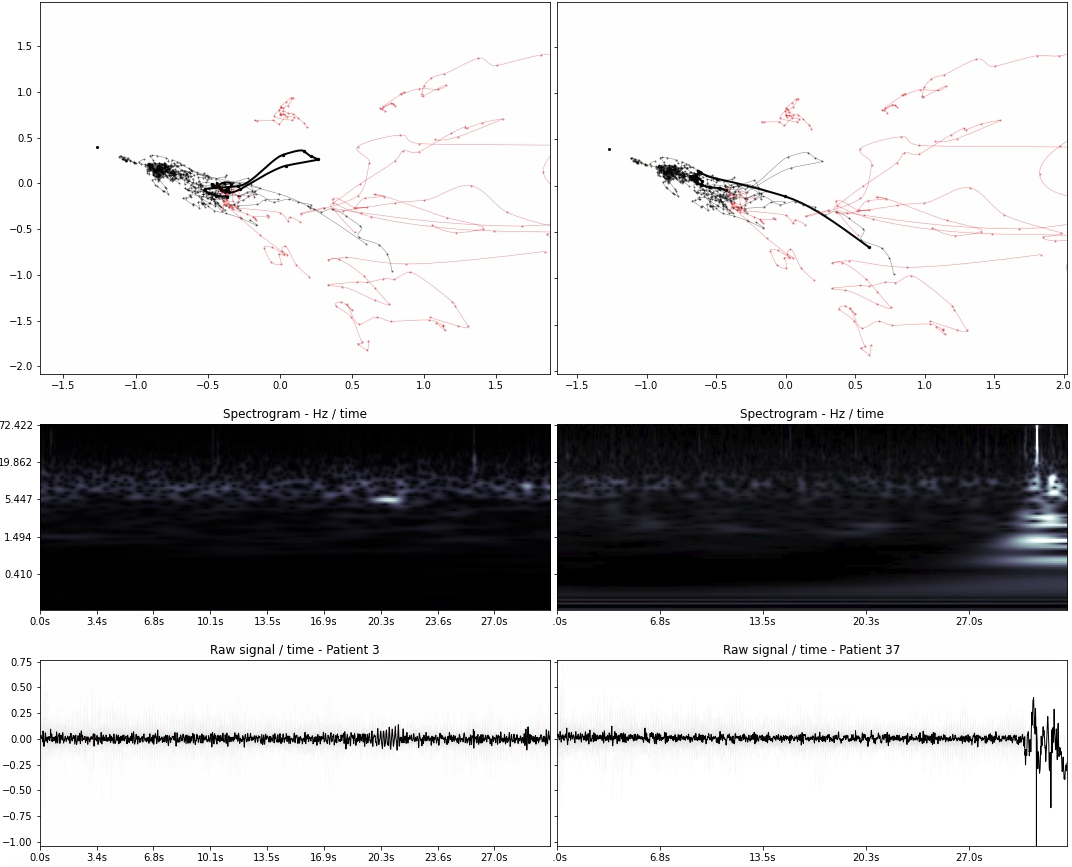
\includegraphics[width=\linewidth]{figures/nemo/exp1-337.png}
\caption{Temporary tremors on the left, and premature end of experiment on the right.}
\label{fig:exp1-337}
\end{figure*}


\begin{figure}
\begin{tabular}{cc}
\subfloat[G-PCA]{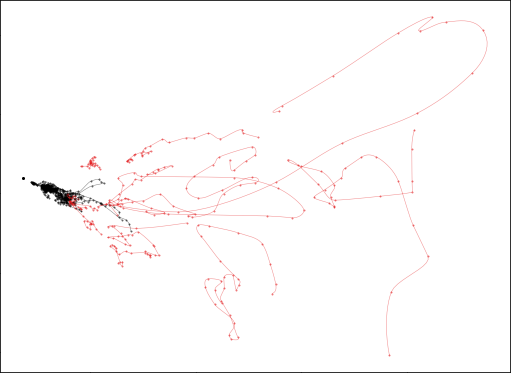
\includegraphics[width=.5\linewidth]{figures/nemo/exp1-5s-window.png}} &
\subfloat[PCD-tSNE $\lambda=.1$]{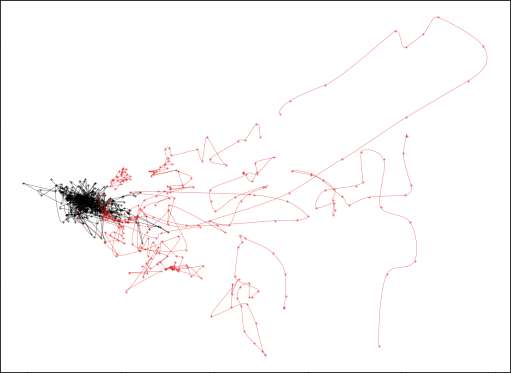
\includegraphics[width=.5\linewidth]{figures/nemo/exp1-pcd0,1.png}} \\
\subfloat[PCD-tSNE $\lambda=.001$]{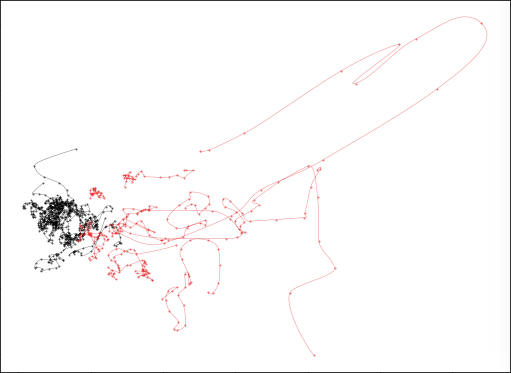
\includegraphics[width=.5\linewidth]{figures/nemo/exp1-pcd0,001.png}} &
\subfloat[PCD-tSNE $\lambda=.0001$]{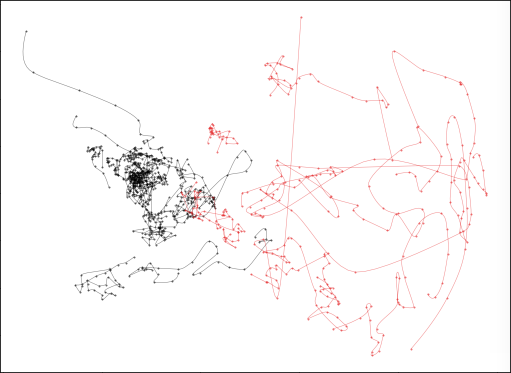
\includegraphics[width=.5\linewidth]{figures/nemo/exp1-pcd0,0001.png}}\\
\subfloat[PCD-tSNE $\lambda=.000001$]{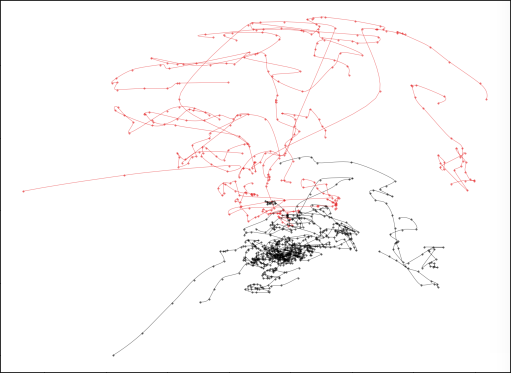
\includegraphics[width=.5\linewidth]{figures/nemo/exp1-pcd0,000001.png}} &
\subfloat[G-tSNE]{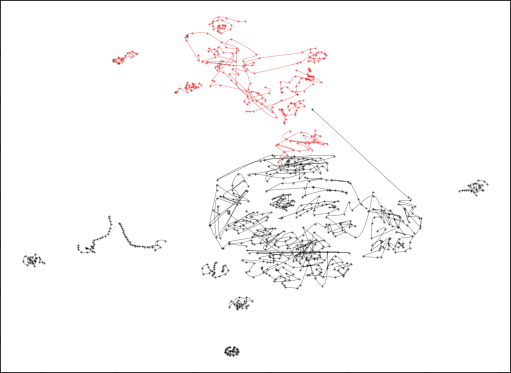
\includegraphics[width=.5\linewidth]{figures/nemo/exp1-gtsne.png}}
\end{tabular}
\caption{}
\end{figure}


\section{Discussion}

\section{Conclusions}


    
